\documentclass[a4paper]{article}
\usepackage[utf8x]{inputenc}  % si utf8
\usepackage{graphicx}

\pagestyle{plain}

\title{\textbf{Game Design Document}\\- \Huge{Incidence} -}
\author{\emph{CHAMBONNET Kevin}\\\emph{GAUTHIER Silvère}\\\emph{MARTINEZ Thierry}\\\emph{MOKHRETAR Amin}}
\date{\today}

\newcommand{\alinea}{\hspace*{0.5cm}}

\begin{document}
  \maketitle
  \newpage
  \tableofcontents

% Liens utiles : 
% http://fr.scribd.com/doc/36304807/Game-Design-Document-Futurn
% http://fr.openclassrooms.com/informatique/cours/redigez-des-documents-de-qualite-avec-latex/memento-2

  \newpage
  \part{Présentation générale}
    \section{Philosophie}
      \alinea Du point de vue d’un observateur, un monde peut être qualifié de complexe sans que les individus y évoluant ne le soient forcément. Dans ce TER, il est question d’aborder cette thématique sous forme de jeu. Autrement dit, le problème qui nous intéresse ici est de déterminer comment faire émerger un comportement global en mettant en oeuvre des contraintes extérieures dans l’environnement pour influencer les interactions locales d’agents. De plus il faudra, pour le joueur, analyser le comportement des ces derniers afin d’optimiser la réalisation des buts demandés. Plus précisément, il s’agit de mettre en scène des agents (disposant d’un comportement précis et défini en terme d’interaction), évoluant dans un environnement modifiable par un joueur humain (qu’il s’agisse d’ajouter des ressources exploitables, de modifier le relief, etc.) devant atteindre un certain objectif (stabilité du système écologique, récolte d’une certaine quantité de ressources, développement d’un chemin).

    \section{Questions fréquentes}
      \subsection{Qu'est-ce que ce jeu ?}
        \alinea C'est un jeu de type God-Like dans lequel on doit aider une civilisation à survivre le plus longtemps possible grâce à différents pouvoirs et actions divines.
			
      \subsection{Qu'est-ce que je contrôle ?}
        \alinea Vous ne contrôlez rien directement, tout se fait de façon indirecte grâce aux pouvoirs. Modifier l'environnement et aider les citoyens sont des actions qu'il faudra effectuer pour faire survivre la civilisation.

%------------------------------------------------------------------------------------

  \newpage
  \part{Mécaniques de jeu}
    \section{Gameplay}
      \subsection{Jouabilité}
        \subsubsection{Conditions de victoire et de défaite}
          \alinea Il n'y aura pas de condition de victoire particulière dans le jeu de base, le but sera de survivre le plus longtemps possible.\\
          La partie se terminera quand le joueur n'aura plus de citoyen.
        \subsubsection{Sauver et Charger une partie}
          \alinea Le joueur pourra sauvegarder sa partie à tout moment, mais la sauvegarde se fera au moment de la dernière nuit.\\
          Le chargement d'une partie placera donc le joueur soit au début de la partie soit à la dernière nuit passée, avec la possibilité de modifier de nouveau les différentes options du jour (météo, métiers...).

%Multijoueur ? Mods ?
%Différent modes de jeu ?
%On peut créer ses propres cartes ? un éditeur accessible ?
%Ajout script, perso, autre ?

	\subsection{Actions du joueur}
      \subsubsection{Pouvoirs de base}
        \begin{itemize} \small
          \item \textbf{Placer un Arbre :} Fait apparaître un Arbre sur une case choisie. Coût : 3 PI.
          \item \textbf{Placer un Arbre Fruitier :} Fait apparaître un Arbre Fruitier sur une case choisie. Coût : 6 PI.
          \item \textbf{Placer de la Pierre :} Fait apparaître de la Pierre sur une case choisie. Coût : 5 PI.
          \item \textbf{Placer de l'Eau :} Fait apparaître de l'Eau sur une case choisie. Coût : 2 PI.
          \item \textbf{Placer une Falaise :} Fait apparaître une Falaise sur une case choisie. Coût : 7 PI.
          \item \textbf{Placer un Buisson :} Fait apparaître un Buisson sur une case choisie. Coût : 4 PI.
          \item \textbf{Placer de la Terre :} Fait apparaître de la Terre sur une case choisie, la Terre placée s'adapte en fonction des autres Terres autour. Coût : 2 PI.
        \end{itemize} \normalsize

      \subsubsection{Pouvoirs divins}
        \begin{itemize} \small
          \item \textbf{Soigner :} Améliore l'état de santé d'un citoyen. Coût : 50 PI.
          \item \textbf{Naissance :} Crée un citoyen supplémentaire, hors naissances quotidiennes. Coût : 200 PI.
        \end{itemize} \normalsize

      \subsubsection{Choix de la nuit}
        \begin{itemize} \small
          \item \textbf{Météo :} Le joueur peut choisir la météo du jour suivant (ensoleillée ou pluvieuse).
          \item \textbf{Métier :} Le joueur peut orienter la distribution des métiers, sans définir exactement la proportion de chaque métier.
        \end{itemize} \normalsize


    \section{Moteur du Jeu}
      \alinea Le moteur du jeu sera divisé en deux parties, le métier et la vue.\\
      L'association de ces deux parties constituera le noyau de l'application, qui communiquera avec les autres modules tels que les Intelligences Artificielles (IA), les fichiers images, les sons... etc.

      \subsection{Moteur multi-agent}
        \alinea La gestion multi-agent se fera à l'aide d'un appel au script de chaque entité pour chaque tick. Chaque entité aura donc un script propre, qui décrira son comportement et pourra faire appel aux primitives que fournira le moteur.

        \subsubsection{Primitives}
          \begin{itemize} \small
            \item Connaître les entités et cases alentours
            \item Connaître l'emplacement du village
            \item Avancer
            \item Changer de direction
            \item Couper un Arbre
            \item Ramasser des Baies
            \item Casser de la Pierre
            \item Cultiver un Champs
            \item Attaquer un animal
            %\item Soigner un Citoyen || Rep. : Pas de healer pour l'instant 
          \end{itemize} \normalsize


        \subsection{Moteur de rendu}
          \alinea L'affichage se fera à base d'un tileset créé entièrement par notre équipe (cf. section \ref{Tuile}, page \pageref{Tuile}).\\
          Le moteur de rendu sera chargé de gérer l'affichage en temps réel de la carte, de ses tuiles ainsi que des entités, afin d'obtenir un résultat fluide.

%------------------------------------------------------------------------------------

  \newpage
  \part{Univers du Jeu}
    \section{La carte}

      \alinea La carte sera composée de 150x150 cases, mais ne sera affiché à l'écran qu'une vingtaine de cases en largeur sur une quinzaine en hauteur. Le déplacement sur la carte pourra se faire grâce aux touches fléchées mais aussi en plaçant la souris sur un des bords de l'écran.\\
      Le joueur ne pourra pas voir au delà des limites des 150x150 cases composant la carte.

    \section{Les Cases}

      \alinea La carte sera découpée en cases. Chaque case aura un type de base en début de partie, qui pourra ensuite être modifié selon le déroulement du jeu (cf. section \ref{DiagCase}, page \pageref{DiagCase}). Un élément neutre est un type de case ne donnant pas lieu à une ressource quelconque.\\
      \newline
      \label{TabCase}
      \begin{small}
        \begin{tabular}{| c | c | c |p{5cm}|}
          \hline
          &  &  &  \\
          \textbf{Type de case} & \textbf{Ressources} & \textbf{Franchissable} & \textbf{Description}\\
          &  &  &  \\
          \hline
          Terre & - & Oui & Type par défaut.\\
          \hline
          Terre Aride & - & Oui & Terre ne pouvant pas être cultivée.\\
          \hline
          Terre Innondée & - & Oui & Terre ne pouvant pas être cultivée.\\
          \hline
          Terre Fertile & - & Oui & Terre pouvant etre cultivée pour devenir un \textbf{Champs}.\\
          \hline
          Champs & Nourriture & Oui & Terre cultivée possédant plusieurs stades de maturité. Le maximum atteint, la récolte peut être effectuée et offrir de la nourriture.\\
          & (1 à 3 unités) &  &  \\
          \hline
          Arbre & Bois & Non & Peut être coupé pour récolter du bois.\\
          & (3 unités) &  &  \\
          \hline
          Arbre Fruitier & Bois, Nourriture & Non & Peut être coupé pour récolter du bois et de la nourriture.\\
          & (2 unités de chaque) &  &  \\
          \hline
          Eau & - & Non & Des poissons peuvent s'y trouver permettant de récolter de la nourriture.\\
          \hline
          Pierre & Pierre & Non & Peut être cassée pour récolter de la pierre.\\
          & (2 unités) &  &  \\
          \hline
          Falaise & - & Non & Elément neutre. Peut faire apparaître de la pierre à ses pieds.\\
          \hline
          Buisson & Nourriture & Non & La récolte de ses baies permet d'obtenir de la nourriture.\\
          & (2 unités) &  &  \\
          \hline
        \end{tabular}
      \end{small}
    
      \subsection{Diagramme de transitions des différentes cases}
        \begin{figure} %problème d'affichage
          \begin{center}
            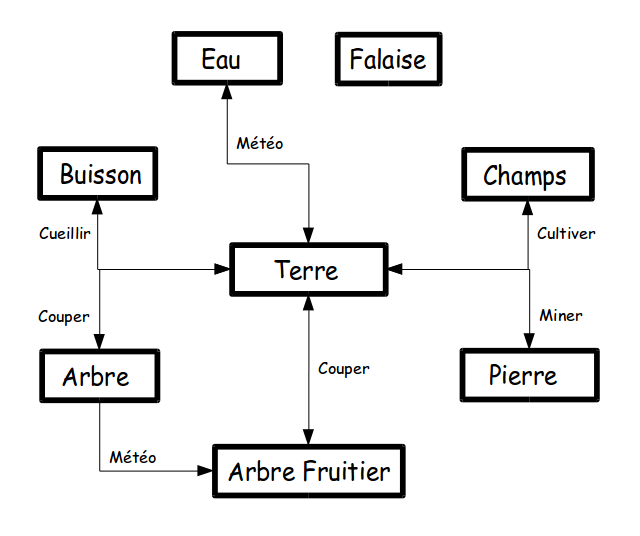
\includegraphics[scale=0.35]{img/DiagrammeTransitionCases.png} 
          \end{center}
          \label{DiagCase}
          \caption{Diagramme de transitions des différentes cases}
        \end{figure}
        
    \section{Ressources}
      \subsection{Ressources utilisées par les citoyens}
        \alinea Ces ressources pourront être stockées dans une quantité illimitée, et les citoyens les utiliseront pour des constructions ou pour se nourrir.
        \begin{itemize} \small
          \item \textbf{Bois :} Utilisé pour la construction des bâtiments.
          \item \textbf{Pierre :} Utilisé pour la construction de certains bâtiments.
          \item \textbf{Nourriture :} Consommé par les citoyens chaque nuit pour se nourrir.
        \end{itemize} \normalsize
        \textbf{Comment ces ressources sont-elles récoltées ? }\\
        \alinea Elles sont récoltées par les citoyens, ainsi chaque métier correspond à la récolte d'une de ces ressources (cf. section \ref{Metier}, page \pageref{Metier}).

      \subsection{Ressources utilisées par le joueur}
        \alinea Cette ressource est la seule que le joueur pourra utiliser, elle sera stockée dans une quantité illimitée.
        \begin{itemize} \small
          \item \textbf{Point d'Incidence (PI) :} Utilisé à chaque action ou pouvoir divin.
        \end{itemize} \normalsize
        \textbf{Comment cette ressource est-elle récoltée ? }\\
        \alinea Elle sera obtenue grâce aux citoyens qui nous en feront gagner une petite quantité tout au long de leur journée. La nuit, chaque citoyen rapporte des points bonus.

%------------------------------------------------------------------------------------

  \newpage
  \part{Les Entités de l'Univers}
    \section{La vie des entités}

      \subsection{Les métiers des citoyens}
        \label{Metier}
        \alinea Chaque citoyen aura une tâche à accomplir durant la journée et ne pourra pas en changer avant la nuit. La nuit, un métier sera attribué à chaque citoyen selon les choix du joueur et les besoins des citoyens (cf. section \ref{Cycle}, page \pageref{Cycle}).
        \begin{itemize} \small
          \item \textbf{Bûcheron :} Coupe les arbres et récolte les ressources associées (Le Bois en général mais aussi de la nourriture sur les Arbres Fruitier).
          \item \textbf{Mineur :} Casse les rochers et récolte la Pierre.
          \item \textbf{Chasseur-Cueilleur :} Chasse les animaux, cueille les baies ou cultive des champs pour récolter la Nourriture.
        \end{itemize} \normalsize

      \subsection{La santé des entités vivantes}
        \alinea Chacune des entités possède une gestion de la santé avec plusieurs états.
        \begin{itemize} \small
          \item \textbf{Bonne santé :} Si l'entité est un citoyen, elle offre de plus grands bonus de PI.
          \item \textbf{Normal :} L'entité est dans son état par défaut.
          \item \textbf{Blessé/Malade :} L'entité agit avec un léger malus de vitesse. Si l'entité est un citoyen, elle offre de plus petits bonus de PI.
          \item \textbf{Gravement blessé/malade :} L'entité agit avec un malus de vitesse plus important. Si l'entité est un citoyen, elle n'offre plus de PI.
          \item \textbf{Mort :} L'entité disparaît.
        \end{itemize} \normalsize
        \begin{figure}
          \begin{center}
            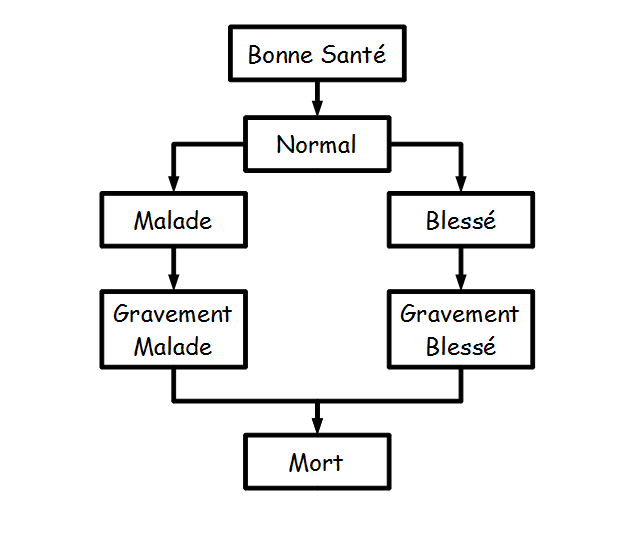
\includegraphics[scale=0.5]{img/DiagrammeTransitionSante.png} 
          \end{center}
          \label{DiagSante}
          \caption{Diagramme de transitions entre les états de santé}
        \end{figure}
        
    \section{Comportement des animaux}
% A FAIRE


    \section{La météorologie}
      \alinea La météo sera présente et sera contrôlée par le joueur. Elle aura une incidence sur l'environnement et les citoyens. Elle sera basique : ensoleillée ou pluvieuse, chacune des deux aura une incidence différente. 
      \begin{itemize} \small
        \item \textbf{Temps ensoleillé :} Améliore la pousse des champs mais un excès de soleil assèche les terres et récoltes, peut réduire les étendues d'eau et une sécheresse trop longue peut faire brûler certaines ressources.
        \item \textbf{Temps pluvieux :} Permet de faire pousser les champs. Un surplus de pluie innonde les terres et récoltes, augmente les probabilités de maladie et peut augmenter la taille des étendues d'eau.
      \end{itemize} \normalsize


    \section{Le cycle jour/nuit}
      \label{Cycle}
      \alinea Un cycle jour/nuit sera présent, avec des journées longues et des nuits courtes. Le Jour, les citoyens se vouent à leur métier, jusqu'au soir. La Nuit, tous les citoyens retournent au village, plus aucune action n'est possible. Lorsque la nuit tombe, toutes les actions du jour ont une incidence sur la nature et les entités, et seront visibles au début de la nouvelle journée.
      \begin{itemize} \small
        \item Le terrain est mis à jour, toutes les actions de la journée auront une incidence sur l'environnement.
        \item Tous les citoyens se nourrissent, la nourriture diminue en fonction du nombre de citoyen \textit{(-3 de nourriture par citoyen)}. S'ils manquent de la nourriture, certains citoyens peuvent tomber malade.
        \item Certains citoyens tombent malade en fonction des anciennes météos.
        \item S'il y a assez de nourriture, de nouveaux citoyens peuvent naître.
        \item Gain des points bonus d'incidence en fonction de la taille de la population et de sa santé.
        \item Mise à jour du métier de chaque citoyen, choisi en fonction des choix du joueur et des besoins.
      \end{itemize} \normalsize

      \subsection{Les incidences sur l'environnement :}
        \begin{itemize} \small
          \item Une étendue d'eau peut faire apparaître des poissons.
          \item Une étendue d'eau peut faire apparaître de la végétation dans les environs.
          \item Une zone de végétation très dense augmente les chances de faire apparaître des animaux herbivores.
          \item Une grande concentration d'animaux herbivores peut faire apparaître des animaux carnivores.
          \item Une forêt très dense augmente les chances de faire apparaître des arbres fruitiers.
          \item Les falaises peuvent faire apparaître des pierres par éboulement.
          \item La météo peut modifier la taille des étendues d'eau, assécher ou humidifier la terre.
        \end{itemize} \normalsize

%------------------------------------------------------------------------------------

  \newpage
  \part{Effets Visuels}

%Ici c'est tout ce qui touche a l'aspect visuel du jeu (2D, 3D, iso ou pas) Taille des sprites, des croquis, réaliste/rétro/abstrait. Tout ce qui est visuel en gros.

    \section{Les tuiles}
      \label{Tuile}
      \alinea Les tuiles seront des images de 32x32 ou 16x16 pixels au format PNG.\\
      \begin{itemize} \small
        \item \textbf{Le sol :} Il y aura 16 tuiles pour chaque type de sol, correspondant à toutes les possibilités de jonction avec le type voisin. En effet, chaque type de sol ne pourra être en contact qu'avec deux types différents suivant l'ordre hiérarchique suivant :\\
          Eau -> Terre innondée -> Terre fertile -> Terre -> Terre aride
        \item \textbf{Les ressources :} Il y aura 4 tuiles pour chaque ressource, correspondant au type de sol sur lequel elle se trouve.
        \item \textbf{Les bâtiments :} Chaque bâtiment sera constitué d'un ensemble de tuiles.
      \end{itemize} \normalsize
  
    \section{Les entités}
      \alinea Chaque entité aura plusieurs positions possibles. Pour chacun d'elle, un ou plusieurs éléments graphiques seront créés.\\
      \textbf{Les positions basiques :} Face, dos, profil droit, profil gauche.\\
      \textbf{Les positions spécifiques :} Coupant du bois, ramassant des baies, chassant, cultivant, construisant, se déplaçant sans ressource, se déplaçant avec des ressources.
	
	\section{Interface utilisateur}
		%Ici c'est tout ce qui est lié aux boutons et interfaces que le joueur utilisera 
		
%------------------------------------------------------------------------------------

  \newpage
  \part{Effets Sonores}
  
%Comme au dessus mais cette fois-ci pour le son. Bruit des animaux (global(ambiant), local(chaque animal son bruit) ?), musique, effet sonore bruitage.

%------------------------------------------------------------------------------------

  \newpage
  \part{Contrôles du jeu}
  
%Souris/Clavier, Manette, autre ?
%Si souris/clavier, des boutons cliquables pour toutes les actions ? Des raccourcis clavier ? Si oui, lesquels ?
  
\end{document}
